\documentclass[tikz]{standalone}

\usepackage[latin1]{inputenc}
\usepackage{tikz}
\colorlet{myblue}{cyan!40!white}
\usetikzlibrary{quotes,angles,calc,decorations.markings}
% GNUPL
% Draw line annotation
% Input:
%   #1 Line offset (optional)
%   #2 Line angle
%   #3 Line length
%   #5 Line label
% Example:
%   \lineann[1]{30}{2}{$L_1$}
\newcommand{\lineann}[4][0.5]{%
    \begin{scope}[rotate=#2, blue,inner sep=2pt]
        \draw[densely dashed, blue!40] (0,0) -- +(0,#1)
            node [coordinate, near end] (a) {};
        \draw[densely dashed, blue!40] (#3,0) -- +(0,#1)
            node [coordinate, near end] (b) {};
        \draw[|<->|] (a) -- node[] {\contour{white}{#4}} (b);
    \end{scope}
}
\newcommand{\lineannOnly}[4][0.5]{%
    \begin{scope}[rotate=#2, blue,inner sep=2pt]
        \draw[densely dashed, blue!40] (0,0) -- +(0,#1)
            node [coordinate, near end] (a) {};
        \draw[densely dashed, blue!40] (#3,0) -- +(0,#1)
            node [coordinate, near end] (b) {};
        % \draw[|<->|] (a) -- node[] {\contour{white}{#4}} (b);
    \end{scope}
}
\usepackage[outline]{contour}
\contourlength{2.1pt}
\begin{document}
\pagestyle{empty}


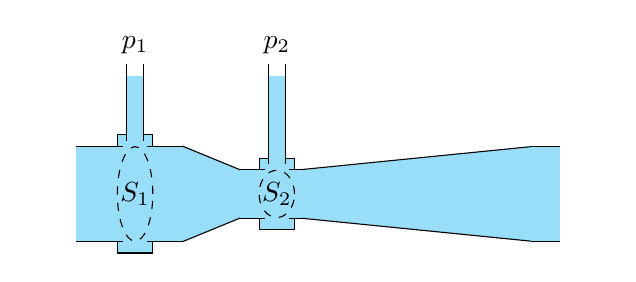
\begin{tikzpicture}[
    scale=1.5, 
    arrowline/.style={black!60},
    kos/.style={black},
    tangent/.style={
        decoration={
            markings,% switch on markings
            mark=
                at position #1
                with
                {
                    \coordinate (tangent point-\pgfkeysvalueof{/pgf/decoration/mark info/sequence number}) at (0pt,0pt);
                    \coordinate (tangent unit vector-\pgfkeysvalueof{/pgf/decoration/mark info/sequence number}) at (1,0pt);
                    \coordinate (tangent orthogonal unit vector-\pgfkeysvalueof{/pgf/decoration/mark info/sequence number}) at (0pt,1);
                }
        },
        postaction=decorate
    },
    use tangent/.style={
        shift=(tangent point-#1),
        x=(tangent unit vector-#1),
        y=(tangent orthogonal unit vector-#1)
    },
    use tangent/.default=1
    ]


% \draw[dashed] (0,0) -- (3,0);
\draw[fill=myblue, draw=none] (1.39,0.41) -- (1.9,0.2) -- (1.9,-0.2) -- (1.39,-0.41) -- cycle;

\draw[fill=myblue] (1-.15,0.5) rectangle (1+.15,-0.5);
% \draw[draw=none,fill=myblue] (0,0.4) rectangle (3,-0.4);

\draw[double=myblue, double distance=1.2cm] (0.5,0) -- (1,0);
\draw[double=myblue, double distance=1.2cm] (1.1,0) -- (1.4,0);


\draw (1.4,0.405)  --  (1.9,0.2);
\draw (1.4,-0.405)  --  (1.9,-0.2);

\draw[fill=myblue, draw=none] (1-0.1,0.45) rectangle (1+0.1,-0.45);

\draw[fill=myblue] (2.2-0.15,0.3) rectangle (2.2+0.15,-0.3);
\draw[double=myblue, double distance=0.6cm] (1.89,0) -- (2.1,0);

\draw[fill=myblue, draw=none] (2.4,0.2) -- (4.35,0.4) -- (4.35,-0.4) -- (2.4,-0.2) -- cycle;

\draw (2.4,0.205)  --  (4.35,0.4);
\draw (2.4,-0.205)  --  (4.35,-0.4);

\draw[double=myblue, double distance=1.188cm] (4.35,0) -- (4.6,0);

\draw[double=myblue, double distance=0.6cm] (2.3,0) -- (2.41,0);


\draw[double=myblue, double distance=0.2cm] (1,0.45) --  (1,1) coordinate (temp);
\draw[double distance=0.2cm] (temp) -- ++ (0,0.1) node [above] {$p_1$}; 
\draw[double=myblue, double distance=0.2cm] (2.2,0.25) --  (2.2,1) coordinate (temp);
\draw[double distance=0.2cm] (temp) -- ++ (0,0.1)  node [above] {$p_2$}; 


\draw[dashed] (1,0) node {$S_1$} ellipse (0.15 and 0.4);
\draw[dashed] (2.2,0) node {$S_2$} ellipse (0.15 and 0.2);



\end{tikzpicture}


\end{document}